% -*- root: ../../../main.tex -*-
\subsection{Normal Operation | Log Replication}
In RAFT il \textbf{Leader} è l'unico server in grado di apportare delle modifiche al \textit{log} . Una volta eletto correttamente, inizia a servire tutte le richieste dei client; allo stesso tempo propaga le modifiche al cluster e si assicura che tutti i server replichino la giusta sequenza di comandi, mantenendo così il \textit{log} consistente nell'intero cluster.
Internamente il \textbf{Leader} mantiene tutti le informazioni riguradanti i log di tutti i \textbf{Follower}; questo perche il \textbf{Leader} deve inviare solo'lentry successiva all'ultima registrata dal \textbf{Follower} così da procedere in sequenza.

\begin{figure}[H]
	\centering
	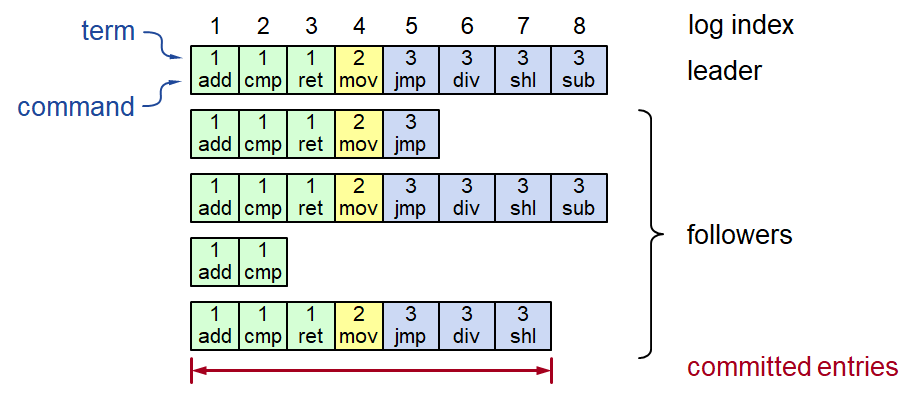
\includegraphics[width=0.80\columnwidth]{raft/logStructure}
	\caption{In figura si evidenzia la struttura del log mantenuto da ognuno dei server. Ogni elemento del log memorizza l'istruzione da eseguire e il term a cui essa appartiene.
		Il log del leader è quello che fa fede in quel dato term e deve essere replicato anche negli altri.
		I log vengono memorizzati sul disco, affinchè possano sopravvivere ai crash della macchina. 
		Se il leader sa che una entry è stata replicata sulla maggiorparte dei server, allora essa passa allo stato di "committed" e può essere eseguita in maniera sicura dalle macchine a stati.}
	\label{fig:figure5}
\end{figure}
Il \textbf{Leader} è l'unico punto di comunicazione con i \textit{client} in tutto il cluster. Ogni richiesta da parte dei \textit{client} contiene almeno un comando, che il \textbf{leader} aggiunge al proprio \textit{log} come nuova entry, e che poi propaga tramite l'invio di più \textit{AppendEntries}.
Una volta che il \textbf{Leader} ha ricevuto la maggior parte degli ack da parte dei \textbf{Follower}, considera sicura l'esecuzione di tale entry(esegue il \textit{commit} dell'entry); esegue la sequenza di comandi e invia il risultato al \textit{Client}.
Parallelamente il \textbf{Leader} procede alla propagazione dell'avvenuto commit su tutto il cluster; ogni \textit{Follower} procederà quindi alla registrazione dell'commit, alla sua esecuzione e infine invierà un ack verso il leader.
\\
Il \textbf{Leader} mantiene traccia dell'ultima entry che è stata validata,e include il suo indice e term in tutte le \textit{AppendEntries}(inclusi gli \textit{heartbeats}) per comunicarla a tutti i \textbf{Follower} e fare l'\textit{append} dell'\textit{entry}.
L'operazione di append ha successo solo nel caso in cui ci sia corrispondenza tra l'elemento precedente del log del leader e l'elemento nella stessa posizione, del log del follower. 
\begin{figure}[H]
	\centering
	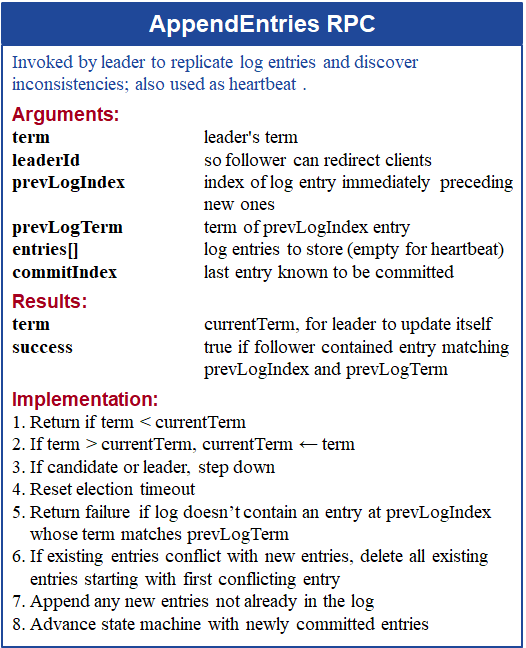
\includegraphics[width=0.80\columnwidth]{raft/appendEntries}
	\caption{Il leader replica il proprio log inviando un elemento per volta al log dei vari follower, i quali accettano solo se c'è corrispondenza tra l'entry precedente a quella inviata dal leader e la loro ultima entry.}
	\label{fig:figure6}
\end{figure}

Se questo non accade, l'operazione fallisce e il \textbf{Leader} invia l'\textit{entry} precedente all'ultima inviata; se anch'essa non corrisponde, invia quella ancora prima e così via, fino a trovare una corrispondenza, come in figura \ref{fig:figure7} \textbf{Follower a}.
Questa operazione si basa sul fatto che se due entry di due diversi server corrispondono, ovvero hanno lo stesso indice, lo stesso term e, di conseguenza, lo stesso comando, allora anche tutte le precedenti entry dei due log sono tra di loro equivalenti.

\begin{figure}[H]
	\centering
	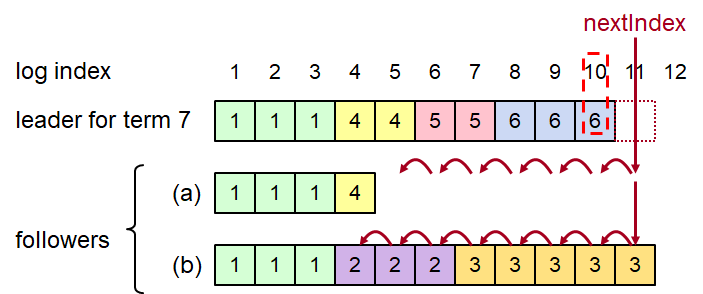
\includegraphics[width=0.80\columnwidth]{raft/repairingFollowerLogs}
	\caption{Il leader procde ad inviare entry con indice sempre minore fino a trovare una corrispondenza, per poi risalire fino alla cima del log, se necessario sovrascrive le entry inconsistenti del Follower.
	\\
	In figura, il leader deve inviare la entry in posizione 10, con term 6.
	\\
	Nel caso a) l'indice 10 è vuoto, di conseguenza il leader procede a ritroso finchè non trova corrpondenza all'indice 4.
	\\
	Nel caso b) all'indice 10 c'è una entry diversa da quella del leader, di conseguenza esso procede a ritroso fino all'indice 3, dal quale inizierà a ricostruire il log sovrascrivendo le entry inconsistenti.
}
	\label{fig:figure7}
\end{figure}


Il \textbf{Leader} continua ad inviare \textit{AppendEntries} ai \textbf{Follower} che non rispondono, fino a quando non ottiene successo; una eventuale presenza minoritaria di \textbf{Follower} lenti o bloccati non intacca le performance del cluster e non rallenta la validazione di nuove entry da parte del \textbf{Leader}
